\chapter{Лабораторная работа 5}
\section*{Практическое задание}

Целью лабораторной работы №5 является освоение возможностей программы Microsoft Project по управлению финансовыми потоками на основе анализа затрат.

\textbf{Содержание проекта:} команда разработчиков из 16 человек занимается созданием карты города на основе собственного модуля отображения. Проект должен быть завершен в течение 6 месяцев. Бюджет проекта: 50 000 рублей.

Команда проекта состоит из 5 программистов (из них 1 ведущий), Web-дизайнера, системного аналитика, 5 наборщиков данных, 2 дизайнеров, технического писателя и медиа-корреспондента.

Все задачи со сроком завершения до 15 мая были отмечены как выполненные, со следующими исключениями: фактическая длительность задачи №5 была увеличена на 20 процентов (с 16 до 20 дней), дата завершения задачи №15 была установлена на 22 апреля, процент выполнения задачи №10 был установлен на 80 процентов.

Помимо этого использование сервера стало осуществляться на безвозмездной основе, а к затратам проекта прибавилось 3200 рублей согласно договору от 1 апреля об оказании организацией-партнёром сервисных услуг до конца проекта.

С 1 апреля ведущий программист был отправлен на курсы повышения квалификации на 2 недели, для этого была изменена доступность ресурса (в течении обучения доступность ведущего программиста снижена вдвое).

Также с 11 апреля совещания были заменены презентации, проходящие раз в 2 недели. Каждая презентация длится 2 часа, на ней присутствуют ведущий программист, мультимедиа-корреспондент, системный аналитик и Web-дизайнер. Также на каждой презентации используется по 0.5 пачки бумаги (1 пачка бумаги стоит 100 рублей), а также 6 бутылок воды (1 бутылка стоит 40 рублей).

\subsection*{Задание 1}

Согласно полученному заданию была задана дата отчёта 15 мая (Проект, Состояние, Дата отчёта о состоянии):
\begin{figure}[h!]
	
\includegraphics[scale=1, center]{lab04_task1_1}
\end{figure}

Была отображена таблица затрат (Вид, Таблицы, Другие таблицы, Освоенный объём), в неё были добавлены столбцы с индексом отклонения стоимости и индексом отклонения от календарного плана (ИОС и  ИОКП):

\begin{figure}[h!]
	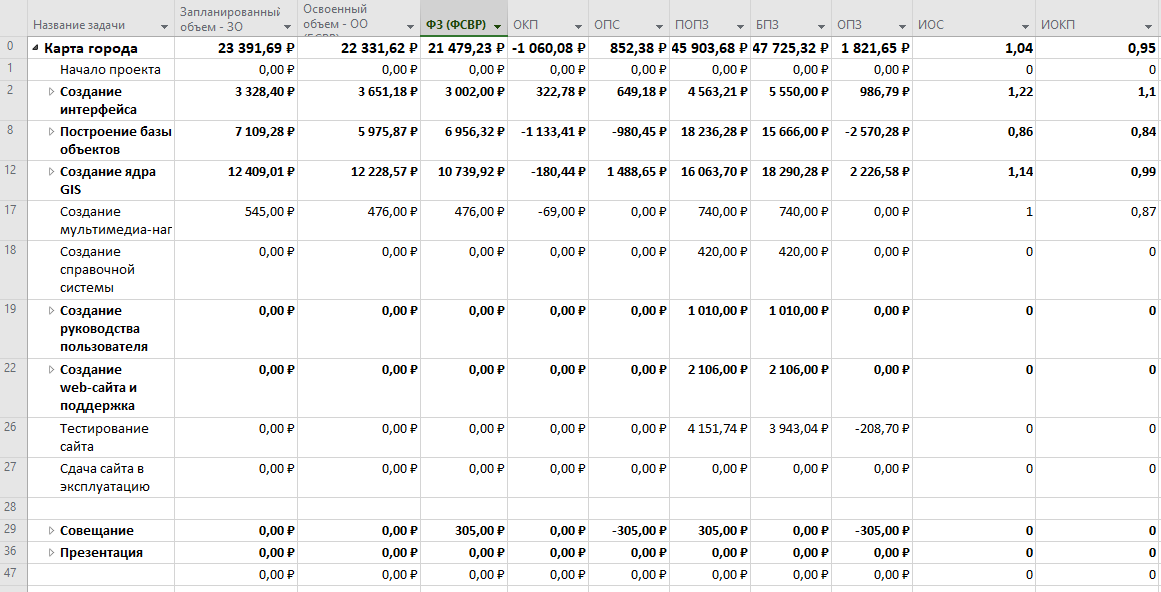
\includegraphics[scale=0.4, center]{lab05_task1_2}
\end{figure}

\clearpage

К 15 мая освоенный объём составляет 22 331 рубль, что почти на тысячу рублей меньше запланированного (23 391 рубль), это происходит из-за того, что задача 8 идёт с отставанием (задача 10 выполнена лишь на 80 процентов).

Фактические затраты же составили 21 479 рублей, что меньше освоенного объёма из-за того, что частые совещания были заменены более редкими и дешёвыми презентациями.

ОКП отрицателен (-1 060 рублей), что означает, что проект несколько запаздывает по сравнению с планом.

ОПС положителен (852 рубля), что означает, что проект укладывается в смету.

ОПЗ положителен (1 821 рубль), что означает, что нет перерасхода средства. 

О том же говорят и коэффициенты ИОС (1.04) и ИОКП (0.95).

Не смотря на запаздывание проекта по сравнению с планом, дата завершения всё ещё укладывается в сроки (16 августа).


\subsection*{Задание 2}

Был создан отчёт о бюджетной стоимости (Отчёты, Наглядные отчёты, Отчёт о бюджетной стоимости):

\begin{figure}[h!]
	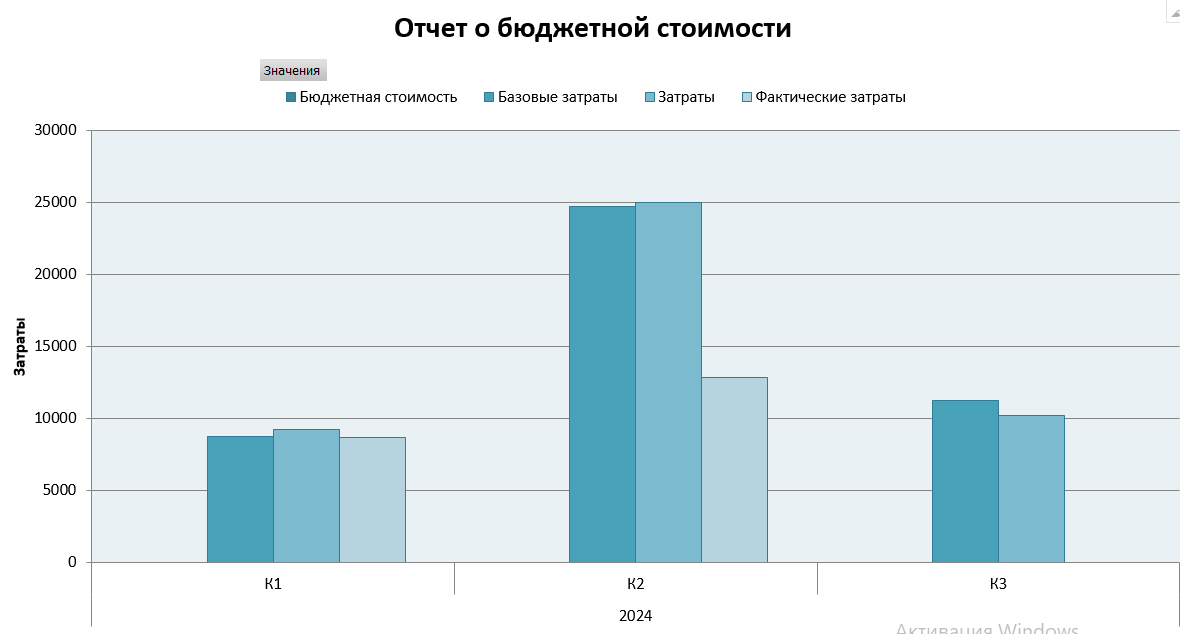
\includegraphics[scale=0.4, center]{lab05_task2_1}
\end{figure}

На вкладке использования назначений можно посмотреть затраты по неделям:
\begin{figure}[h!]
	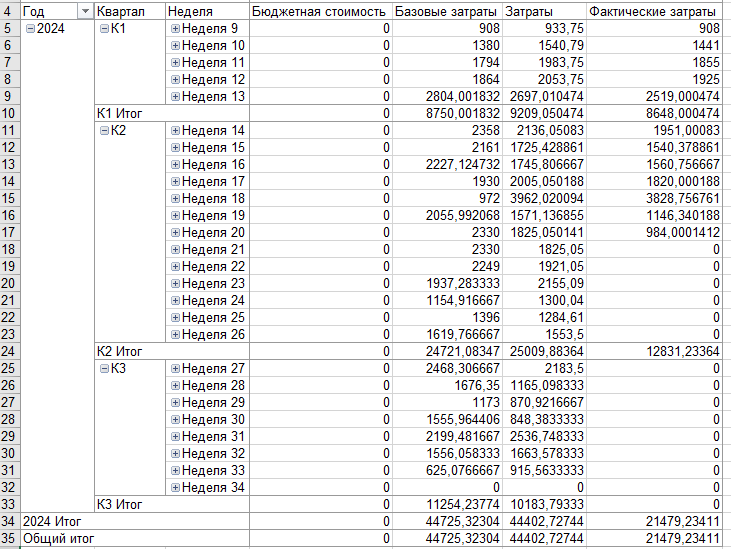
\includegraphics[scale=0.4, center]{lab05_task2_2}
\end{figure}

\begin{figure}[h!]
	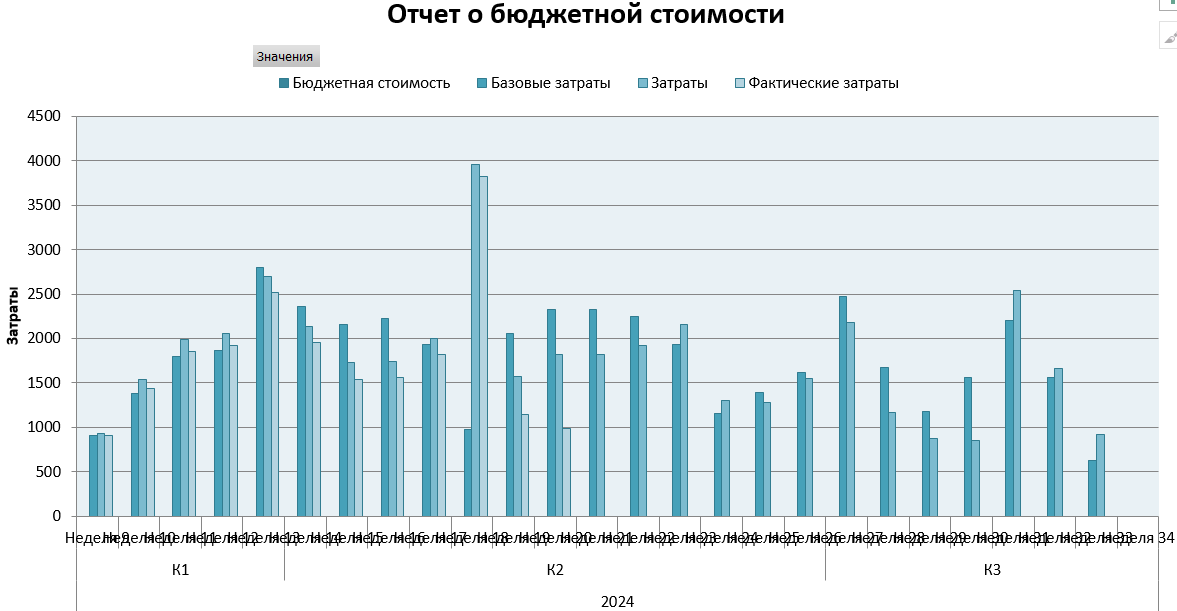
\includegraphics[scale=0.4, center]{lab05_task2_3}
\end{figure}

Видно, что наибольшее число денег понадобится на неделе 18. В это время выполнялись задачи ''Программирование средств обработки'', ''Создание модели ядра'', ''Создание рабочей версии модели ядра'', а также ''Создание мультимедиа-наполнения''.

Проанализируем превышение затрат (Отчёт, Затраты, Превышение затрат):

\begin{figure}[h!]
	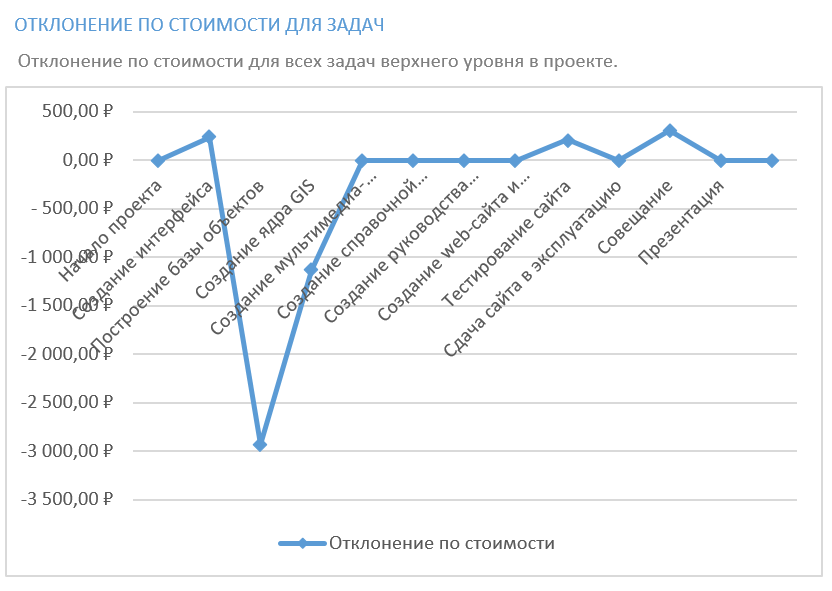
\includegraphics[scale=0.5, center]{lab05_task2_4}
\end{figure}

\begin{figure}[h!]
	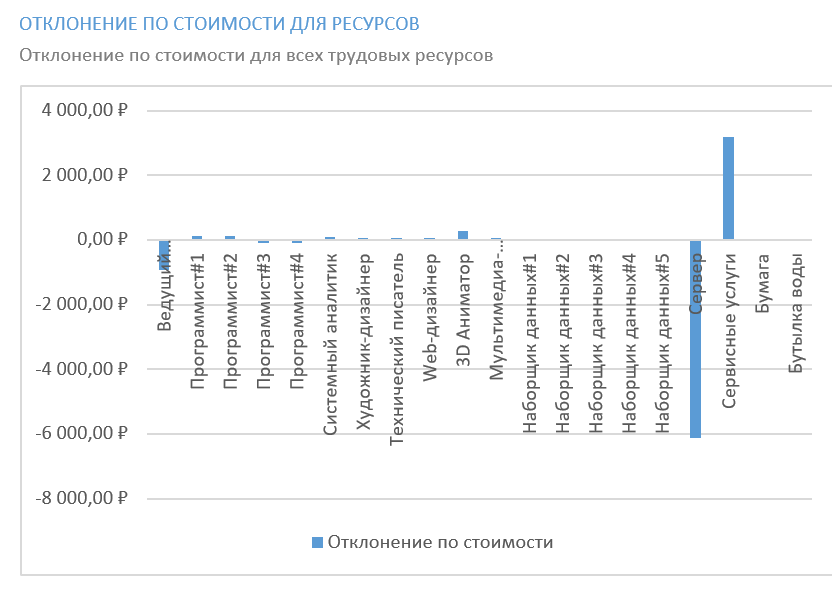
\includegraphics[scale=0.5, center]{lab05_task2_5}
\end{figure}

\clearpage

Отклонения присутствуют у создания интерфейса (поскольку длительность задачи 5 была увеличена на 20 процентов), у создания ядра GIS, поскольку ведущий программист работал меньше и его заменили более дешёвые программисты, у тестирования сайта (поскольку зарплата ведущего программиста стала больше).

Для ресурсов наиболее сильные отклонения возникли для ведущего программиста (в меньшую сторону, т.к. пока он поднимал квалификацию, он работал лишь на половину ставки), а также для сервера и сервисных услуг.


\subsection*{Задание 3}

Был взят файл с результатами лабораторной работы №2, задачи были декомпозированы, за основу были взяты этапы жизненного цикла ПО: анализ, проектирование, разработка, тестирование и поддержка.

Вот состояние проекта до и после декомпозици:

\begin{figure}[h!]
	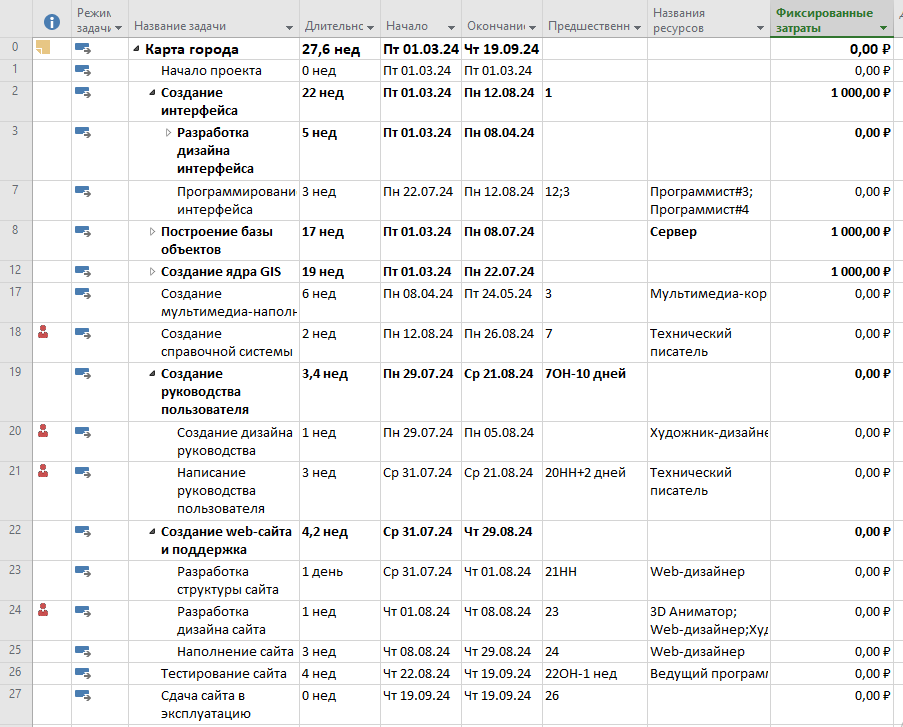
\includegraphics[scale=0.51, center]{lab05_task3_1}
\end{figure}

\begin{figure}[h!]
	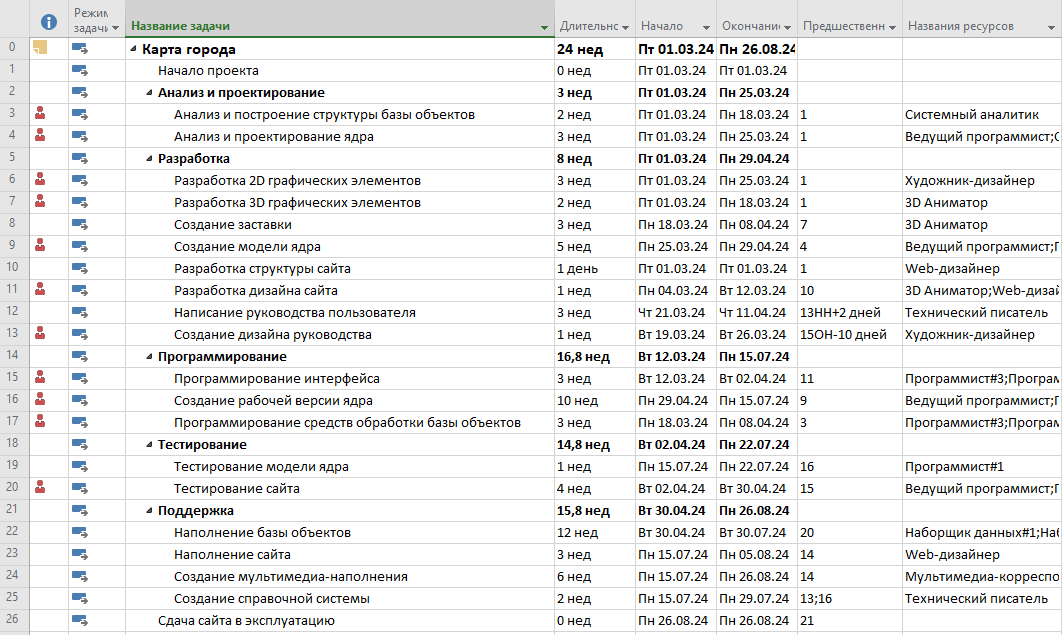
\includegraphics[scale=0.4, center]{lab05_task3_2}
\end{figure}


Несмотря на то, что дата окончания проекта стала 26 августа против 19 сентября, в каждом этапе жизненного цикла ПО, кроме поддержки, есть перегрузки, поскольку исполнители вынуждены делать несколько задач одновременно: так, во время разработки, художник-дизайнер должен одновременно делать дизайн руководства и разработку 2D элементов. Необходимо производить выравнивание, после которого дата окончания проекта точно выйдет за рамки установленных 6 месяцев.

Декомпозиция задач проекта, сделанная на основе жизненного цикла ПО, является альтернативным способом декомпозиции задач, который при проведении выравнивания и устранении перегрузок может заменить способ, выбранный ранее.

\section*{Заключение}

В ходе выполнения данной лабораторной работы были отработаны навыков использования программы Microsoft Project для управления финансовыми потоками.

На 15 мая проект запаздывает по сравнению с планом, однако укладывается в смету (перерасход средств отутствует) и всё ещё укладывается в заложенные 6 месяцев (дата завершения проекта 16 августа).